\documentclass{VUMIFPSbakalaurinis}
\usepackage{algorithmicx}
\usepackage{algorithm}
\usepackage{algpseudocode}
\usepackage{amsfonts}
\usepackage{amsmath}
\usepackage{bm}
\usepackage{caption}
\usepackage{color}
\usepackage{float}
\usepackage{graphicx}
\usepackage{listings}
\usepackage{subfig}
\usepackage{wrapfig}
\usepackage{multirow}

% Titulinio aprašas
\university{Vilniaus universitetas}
\faculty{Matematikos ir informatikos fakultetas}
\department{Programų sistemų bakalauro studijų programa}
\papertype{Bakalauro baigiamasis darbas}
\title{Šilumos laidumo uždavinio lygiagretinimo tyrimas naudojant centrinius ir grafinius procesorius}
\titleineng{Steady-state heat equasion parallization analysis on CPU and GPU}
\author{Mantas Petrikas}
\reviewer{lekt. Irus Grinis}
\supervisor{dr. Rokas Astrauskas}
\date{Vilnius – \the\year}

% Nustatymai
% \setmainfont{Palemonas}   % Pakeisti teksto šriftą į Palemonas (turi būti įdiegtas sistemoje)
\bibliography{bibliografija}

\begin{document}
\maketitle


\sectionnonumnocontent{Santrauka}

Šiame nagrinėjamos šilumos laidumo uždavinio lygiagretino galimybes naudojant centrinius ir grafinius procesorius.
Darbo metu buvo implentuoti centrinius procesorius naudojantys nuoseklusis ir lygiagretusis algorimtai bei grafinius procesorius naudojantis algoritmas.
Algoritmus įgyvendinančios programos buvo testuojamos Vilniaus Universiteto Matematikos ir Informatikos fakulteto Skaitmeninių tyrimų ir skaičiavimų centro paskirstytų skaičiavimų tinkle.
Centrinius procesorius naudojanti lygiagretujį algoritmą įgyvendinanti programa buvo ištestuota naudojant 256 branduolius ir buvo gautas 98 kartų pagreitėjimas.
Grafinius procesorius naudojanti lygiagrečioji programa buvo ištestuota naudojant NVIDIA Tesla V100 SXM2 grafinę plokštę ir buvo gautas 360 kartų pagreitėjimas lyginant su nuosekliuoju algorimtu.
Nustatyta, kad grafinius procesorius naudojanti šilumos lygi sprendžianti programa naudoja mažiau elektros energijos resursų nei centrinius procesorius naudojanti programa.


\raktiniaizodziai{Šilumos lygtis, Laplaso lygtis, Centrinis procesorius, OpenMPI, Grafinis procesorius , CUDA}

\sectionnonumnocontent{Summary}

This work examines the parallelization possibilities of the heat transfer problem using CPUs and GPUs.
Serial and parallel algorithms using CPU and algorithm using GPU were implanted during the work.
The program that implement the algorithms were tested in the distributed computing network of the Digital Research and Computation Center of the Faculty of Mathematics and Informatics of Vilnius University.
A program implementing a parallel algorithm using CPUs was tested using 256 cores and speedup of 98 was observed .
A parallel program using graphics processors was tested using an NVIDIA Tesla V100 SXM2 graphics card and the process was 360 times faster to the serial algorithm.
Also, this work constitrutes that an application that solves heat equation uses a graphics processor uses less power than an application that uses a central processing unit.
\keywords{Heat equation, Laplace equation, CPU, OpenMPI, GPU, CUDA}

\tableofcontents


\sectionnonum{Įvadas}

Kompiuterinės simuliacijos yra svarbi modernių tyrimų dalis. 
Norint elektyviai atlikti sudėtingas simuliacijas, dažnai neužtenka vieno kompiuterio branduolio resursų, ir reikia paskirstyti užduoties sprendimo darbą kelioms procesoriaus gijoms, kurios sugebėtų vienu metu, lygiagrečiai atlikti skaičiavimus.
Tai galima padaryti išnaudojant centriniam procesoriuje esančius branduolius ir gijas, naudojant grafinius procesorius, ar pasitelkiant superkompiuteriuose esančius sujungtus mazgus, taip išnaudojant daugiau nei vieną centrinį ar grafinį procesorių.

Viena tipinė lygiagretinimo užduotis yra šilumos lygties sprendimas. 
Šilumos lygtis yra vienas iš Puasono lygties (ang. Poisson's equation) pritaikymo galimybių. 
Šios dalinės diferencialinės lygtys plačiai naudojamos fizikoje, sprendžiant elektrostatikos \cite{house2008analytic}, gravitacijos, magnetizmo \cite{blakely1996potential}, pastovios būsenos temperatūrų \cite {berntsson2001numerical} ir hidrodinamikos \cite{kadanoff1985simulating} problemas. 
Ši dalinė diferencialinė lygtis turi kelis sprendimų būdus, kurių vienas yra naudojant baigtinių skirtumų metodą (ang. finite difference method) \cite{yoon2015analyses}.
Šis metodas leidžia apskaičiuoti šilumos pasiskirstymą tam tikrame apribotame plote, žinant ploto kraštinių taškų temperatūrą.
Norint efektyviau apskaičiuoti temperatūros pasiskirstymą plote, galima pradinį plotą suskirstyti į dalis, ir vykdyti temperatūros skaičiavimus atskirtuose plotuose lygiagrečiai.
Šis darbas nagrinėja šilumos lygties sprendimo galimybes, naudojant centrinius procesorius (ang. CPU) ir grafinius (ang. GPU) lygiagrečiam lygties spręndimui apribotame plote, ir palygina lygiagrečiųjų algoritmų pagreitėjimą ir efektyvumą. 

Darbo tikslas - įvertinti ir palyginti šilumos laidumo uždavinio lygiagretinimo algoritmo galimybes naudojant centrinius ir grafinius procesorius.

Darbo uždaviniai:
\begin{itemize}
    \item implementuoti nuoseklųjį algoritmą, sprendžianti šilumos pasiskirstymo uždavinį
    \item implementuoti nuseklu ir įvertinti šilumos laidumo uždavinio algoritmo pagreitėjimą naudojant centrinius procesorius
    \item suprojektuoti ir implementuoti šilumos laidumo uždavinio sprendimo algorimtą, naudojantį grafinių procesorių resursus
    \item įvertinti grafinius procesorius naudojančio algoritmo našumą ir praktiškumą lyginant su centrinius procesorius naudojančiu algoritmu
    \item palyginti gautus rezultatus rezultatus su kitais panašiais problemas nagrinėjančių mokslinių darbų rezultatais
\end{itemize}

Darbo rezultatai:
\begin{itemize}
    \item Nuoskelioji šilumos laidumo uždavinio sprendimo implementacija
    \item Lygiagrečioji šilumos laidumo uždavinio algoritmo sprendimo naudojanti centrinius procesorius
    \item Lygiagrečioji laidumo uždavinio sprendimo implementacija naudojanti grafinius procesorius
    \item Algoritmų teorinių ir praktinių pagreitėjimų analyzė
    \item Grafinius ir centrinius procesorius naudojančių algoritmų pagreitėjimų palyginimas
\end{itemize}

% Įvade apibūdinamas darbo tikslas, temos aktualumas ir siekiami rezultatai. Darbo įvadas neturi
% būti dėstymo santrauka. Įvado apimtis 1–2 puslapiai.



\section{Šilumos laidumo uždavinys}



Šio darbo tyrimo objektas - šilumos laidumo lygties \cite{burden2011numerical} sprendimo būdai. 


Šilumos pasiskirstymą erdvėje aprašo Puasono lygtis dvimatei erdvei:

\begin{equation}
    \frac{∂^2 u}{∂ x^2}(x,y)+\frac{∂^2 u}{∂ y^2}(x,y) = f(x,y) 
\end{equation}

Kadangi šiame darbe bus nagrinėjamas erdvė be papildomų vidinių šilumos šaltinių, todėl $f(x,y) = 0 $, o temperatūros pasiskirstymą lemia kraštinių taškų temperatūra.
\begin{equation}
    \frac{∂^2 u}{∂ x^2}(x,y)+\frac{∂^2 u}{∂ y^2}(x,y) = 0
\end{equation}
Ši lygtis dar yra žinoma kaip Laplaso lygtis (ang. Laplace's equation).
Norint šia lygtį pritaikyti praktikoje, naudodami baigtinių skirtingų metodą apibrėžiame erdvę - matricą, kurioje bus skaičiuojama temperatūra, pradinę sistemos temperatūra šoniniuose ir vidiniuose taškuose.
Šiame rašto darbe nagrinėjamas temperatūros pasiskirstymą kvadratinėje erdvėje, kurią suskirstysime į vienodo dydžio kvadratinius taškus, turinčius savo temperatūrą.

Naudodami baigtinių skirtumų metodą galime apibrėžti antros eilės dalinės diferencialinės lygties apytikslias reikšmes:
\begin{equation}
    \frac{∂^2 u}{∂ x^2}(x,y) \approx \frac{u(x+h,y)-2u(x,y)+u(x-h,y)}{h^2}
\end{equation}
\begin{equation}
    \frac{∂^2 u}{∂ y^2}(x,y) \approx \frac{u(x,y+h)-2u(x,y)+u(x,y-h)}{h^2}
\end{equation}

kur $h$ yra atstumas tarp taškų, o $u_{x,y}$ - taško temperatūra taške, $x,y$.  
Įstatydami šias reikšmes į Laplaso lygtį gauname:

\begin{equation}
    \frac{u(x+h,y)-2u(x,y)+u(x-h,y)}{h^2} +  \frac{u(x,y+h)-2u(x,y)+u(x,y-h)}{h^2}  = 0 
\end{equation}
\begin{equation}
    \frac{u(x+h,y)+u(x-h,y)+u(x,y+h)+u(x,y-h)-4u(x,y)}{h^2} = 0
\end{equation}
\begin{equation}
    \frac{u(x+h,y)+u(x-h,y)+u(x,y+h)+u(x,y-h)}{h^2} = \frac{4u(x,y)}{h^2}
\end{equation}

Kadangi atstumas šiame darbe nagrinėjame uždavinyje atstumas tarp erdvės taškų nėra lygus 0, galime lygties abi puses padauginti iš $h^2$:


\begin{equation}
    u(x+h,y)+u(x-h,y)+u(x,y+h)+u(x,y-h) = 4u(x,y)
\end{equation}

\begin{equation}
    \frac{u(x+h,y)+u(x-h,y)+u(x,y+h)+u(x,y-h)}{4} = u(x,y)
\end{equation}

Šią formulę galime pritaikyti praktiškai, dvimatę erdvę projektuodami kaip matrica, padalinę ją į vienodo atstumo taškus:
\begin{equation}
    u_{x, y} = \frac{u_{x+1,y}+u_{x-1,y}+u_{x,y+1}+u_{x,y-1}}{4}
\end{equation}

Gauname, kad vidinio taško temperatūros reikšmė yra lygį jį supančių 4 taškų temperatūrų reikšmių vidurkiui (\ref{img:5point} paveikslėlis). 

\begin{figure}[H]
    \centering
    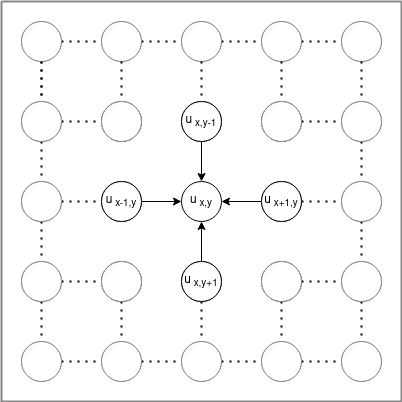
\includegraphics[scale=0.7]{img/5point.png}
    \caption{Temperatūros pasiskirstymas vidiniuose matricos taškuose}
    \label{img:5point}
\end{figure}

Norėdami išspręsti šias lygčių sistemas, naudosime Jakobi iteracinį metodą \cite{burden2011numerical}, kiekvienos iteracijos metu formulės kintamųjų reiškmes keisdami praėjusios iteracijos reikšmėmis.
Laikysime, kad sistema pasiekė galutinę savo būsena, kai tų pačių taškų temperatūrų skirtumai skirtingų iteracijų metu bus mažesni už norima paklaida.

Kraštinių taškų temperatūros pasiskirstymas nulemia galutinį temperatūros pasiskirstymą erdvėje.
Vidinių taškų pradinis temperatūros pasiskirstymas įtakos galiniam temperatūros pasiskirstymui neturi, tačiau gali turėti įtakos konvergencijos greičiui.
Kraštinių taškų temperatūra šito tyrimo metu aprašomą kaip:

\[ f(x, 0) = f(x, N-1) = |sin(x/N \times 2\pi \times 5/2)| = |sin(\frac{5\pi \times x}{N})| \], 

kur N yra matricos kraštinės taškų skaičius.
Ši formulė pirmajai ir paskutinei eilutei priskiria 5 $sin$ bangų teigiamas reikšmes.
Likusiems taškams priskiriama 0 temperatūros reikšmė.
Šio darbo metu taškams priskiriamos temperatūros reikšmės nuo 0 iki 1 imtinai, taip leidžiant modeliuoti į realia objekto temperatūra taikant paprasta proporcija.
Vizualiai pradinis temperatūrų pasiskirstymas matomas \ref{img:start} paveikslėlyje.
Juodi taškai atitinka 1 reikšmę, balti - 0.
Uždavinio tikslas - nustatyti galutinį temperatūros pasiskirstymą plokštelėje, kai temperatūra plokštelėje nebekinta.
Leistina paklaida (temperatūros skirtumas kuri pasiekus laikysime kad programa pasiekė galutinę savo būseną) šio tyrimo eksperimentų metu buvo 0.000001.  
Vizualiai galutinis temperatūros pasiskirstymas matomas \ref{img:end} paveikslėlyje.
Laikas per kurį temperatūra pasiskirsto erdvėje ir erdvė sudarančios medžiagų šiluminis laidumas šiame darbe nėra nagrinėjami. 

\begin{figure}[H]
    \centering
    
\includegraphics[scale=0.7]{img/image_0000000.png}
    \caption{Pradinis temperatūros pasiskirstymas}
    \label{img:start}
\end{figure}

\begin{figure}[H]
    \centering
    
\includegraphics[scale=0.7]{img/image_1000000.png}
    \caption{Galutinis temperatūros pasiskirstymas plokštelėje}
    \label{img:end}
\end{figure}


\section{Lygiagretiems skaičiavimams naudojama įranga}
Šiame skyriuje apžvelgsime įvairius lygiagreties skaičiavimams naudojamus įrenginius. 
Skaičiavimo įrenginai dažnaiusiai skirtomi į 4 kategorijas: CPU - Centriniai procesoriai, GPU - Grafiniai procesoriai, FPGA - Vartotojų programuojamos loginių elementų matricos ir ASIC - Programos specifiniai grandynų grandinės \cite{nurvitadhi2016accelerating}

Centriniai procesoriai (ang. central processing unit -CPU) - yra bendri procesorius, skirtas įvairioms užduotims atlikti.
Populiariausias įrenginys turintis didžiausią programavimo technolojų įvairove ir todėl leidžiantis lengvai įgyvendinti algoritmus
Dauguma modernių centrinių procesorių savyje turi galimybes vykdyti užduotis skirtingomis gijomis, taip leidžiant atlikti kelias instrukcijas vienu metu.


Grafiniai procesoriai (ang. graphic processing unit - GPU) yra specializuotas įrenginys su patobulintomis matematinio skaičiavimo galimybėmis.
Lyginant su centriniais procesoriais, šie grafiniai procesoriai turi didesnis slankaus kablelio skaičiavimo galimybes.
Grafiniai procesoriai dažniausiai naudojami vykdyti vienai instrukcijos su daug duomenų (angl. single-instruction-multiple-data - SIMD) modelio programas \cite{harish2007accelerating}.

Grafiniai procesoriai dėl savo architektūros apribotą galimų atlikti instrukcijų kiekį, 
Grafinių procesoriai naudojimi kompiuterinės grafikos, matematinių skaičiavimų ir mašininio mokymosi užduotyse \cite{root2016mapd}.



Vartotojų programuojamos loginių elementų matricos (ang. Field Programmable Gate Array - FPGA) yra programuoji lustai, skirti programuoti loginius vartus \cite{monmasson2007fpga}.
FPGA leidžia programuotuojui pritaikyti lustą tam tikrai programai, taip pasiekiant didelį programos greitaveiką su energijos mažais suvartojimo kaštais. 
FPGA naudojami aviacijos, medicinos, dirbtinio intelekto, daiktų interneto, laidinio ir belaidžio tinklo, automobilių pramonėje \cite{monmasson2007fpga, hill2017precision}. 
Pastaruoju metu FPGA pradėjo populiarėti ir tarp debesų kompiuterijos pasiūlymų \cite{skhiri2019fpga}.
Nors jų galimybės teoriškai yra identiškos centriniams ir grafiniams procesoriams \cite{vyazigin2021emulation}, dėl naudojamo žemo lygio programavimo kalbų instrukcijų jie naudojami paprastesnėms programoms.

Programos specifiniai grandynų grandinės - (ang. Application-Specific Integrated Circuit - ASIC) yra procesoriai, skirti atlikti vienai specifiniai užduočiai.
Po procesoriaus pagaminimo, jo nebegalima perprogramuoti, todėl jų projektavimui ir testavimui dažniausiai naudojami kitokia aparatinė įranga (dažnai dėl projektavimo panašumo - FPGA).
ASIC naudojami tada kai reikia didelės veikimo spartos, dažniausiai realaus laiko sistemose \cite{genovese2013asic}. 
ASIC tipo lustai pasižymi geriausia greitaveika ir mažiausiais energijos sanaudomis, bet turi didelius proketavimo ir gaminimo kaštus \cite{gayle1993cost}, todėl dažniausiai naudojami industrinėse sferose.

Šiame darbe šilumos pasiskirstymo uždavinys yra sprendžiamas naudojant CPU ir GPU įrenginius. 
Naudojant pagrininius procesorius įgyvenintas nuseklusis ir lygiagretusis algoritmai, o dėl skaičiavimo naudojamos slankaus kablelio aritmetikos lygiagretusis algortimas taip pat bus įgyventintas naudojas grafinius procesorius.     

\section{Algoritmų testavimo metodai}


Siekiant išlaikyti vienodas sąlygas ir ištestuoti algoritmą turint didelį centinių procesorių kiekį, visi šiame darbe aprašyti eksperimentai buvo vykdomi Vilniaus Universiteto Matematikos ir Informatikos fakulteto Skaitmeninių tyrimų ir skaičiavimų centro paskirstytų skaičiavimų tinkle.

Šiame darbe testuoti CPU resursams buvo naudojamas paskirtytų paskirstytų skaičiavimų tinko „beta“ telkinys, kurį sudaro 56 (testavimo metu praktiškai buvo pasiekiami tik 42) mazgai turinys po 2 Intel Xeon X5650 procesorius, kurių kiekvienas turi po 6 branduolius. 
Kiekviename šio telkinio mazge yra 24 GB operatyviosios atminties (ang. RAM) ir jie turi prieigą prie 20Gbit/s infiniband tinklo.
Skaičiavimų tinkle buvo instaliuota Debian operacinė sistemą, lygiagrečiam algoritmui buvo naudojamas OpenMPI bibliotekos 2.1.0 versija.
Programoms paleisti buvo naudojama sistemoje esanti „Slurm“ užduočių valdymo sistema ir „short“ užduočių eilė, turinti 2 valandų ir 2 GB vienam naudojamam branduoliui limitą.

Testuoti GPU resursams buvo naudojamas „hpc“ klasterio „gpu“ telkinys, turintis 3 Tesla V100-SXM2 grafinius procesorius, kiekvienas iš kuriu turi po 32GB operatyviosios atminties, turintis 2560 dvigubos slankiojo kablelio CUDA branduolius.
Skaičiavimų tinkle buvo instaliuota Qlustar 11  operacinė sistemą, sukurta Ubuntu 18.04 LTS pagrindu, gpu testavimui buvo naudota CUDA įrankių 10.1 versija. 
GPU programos paleisti taip pat buvo naudojama sistemoje esanti „Slurm“ užduočių valdymo sistema ir „gpu“ užduočių eilė, turinti 2 valandų ir 12 GB vienam naudojamam branduoliui limitą.
GPU testavimui buvo naudojams tik 1 grafinis procesorius.

Visi programos veikimo laiko testai buvo atliekami po 3 kartus, ir tada buvo parenkamas geriausias programos vykdymo laikas. 
Tai buvo daroma norint išvengti kitų skaičiavimo tinklo naudotojų, sistemos pasileidimo ar laikinų tinklo sutrikimo poveikio testavimo rezultams.

\section{Nuoseklusis algoritmas}

Nuoseklusis algoritmas įgyvendintas C++ kalba. 
Algoritmo pradžioje alokuojama atmintis dviems N*N dydžio masyvams, kur N yra matricos kraštinės ilgis: viename saugoma dabartinė matricos būsena, kitas yra pildomas naujomis reikšmėmis iteracijos metu.
Naudojami vienmačiai masyvai, nes didžioji dalis OpenMPI bibliotekos funkcijų, kuri buvo naudotos lygiagretinant algoritmą, tikisi vienmačių masyvų duomenų perdavimui, o nuoseklaus algoritmo veikimui vienmačių ir dvimačių masyvų naudojimas nedaro didelės įtakos algoritmo veikimo laikui.
Pirmasis masyvas užpildomas pradine matricos būsena, tada pradedamas iteracinis procesas, kai kiekvienos iteracijos metu, kiekvienam vidiniam matricos taškui yra priskiriama reikšmė, lygi jį supančių 4 taškų vidurkiui, o kraštinės matricos reikšmės nekinta.
Taip pat iteracijos metu fiksuojamas maksimalus temperatūros pasikeitimas, skirtas nustatyti ar matrica pasiekė galutinė savo būseną.
Ši reikšmė kiekvienos iteracijos palyginama su nustatyta paklaidos reikšme ir jei temperatūros pasikeitimas yra mažesnis už leistina paklaida, laikome kad matrica pasiekė savo galutinį temperatūrų pasiskirstymą.

Testuojant nuoseklųjį algoritmą su skirtingais matricos kraštinės ilgio reikšmėmis (\ref{table:seq_time} lentelė), nepastebėta tiesioginės sasajos tarp vykdymo laiko ir kraštinės ilgio.
Tačiau fiksuojant iteracijų skaičių, pastėbėta logoritminė priklausomybė tarp programos iteracijų vykdymo laiko ir kraštinės ilgio.
Padidinus kraštinės ilgį beveik 2 kartus, vykdymo laikas padidėja beveik 4 kartus.
Tai galima sieti su tuo, kad algoritmas nagrinėja šilumos pasiskirstymą dvimatinėje erdvėje, todėl padidinus matricos kraštinės ilgį 2 kartus, duomenų kiekis padidėja 4 kartus.
Matricos kraštinės ilgiai pasirinkti dvejeto laipsniai, kad lygiagretinant algoritmą vidinės matricos reikšmes būtų padalinti skirtingiems procesams vienodais kiekiais. 
Į ši skaičių neieina papildomos dvi eilutės, kurios šiame skaičiavime atitinka matricos kraštines - eilutes ir stulpelius kurių temperatūrų reikšmės nekinta.
Testuojant nuoseklųjį algoritmą, kai matricos kraštinę sudaro 2048 taškai, buvo pasiektas sistemos užduočių vykdymo laiko limitas (2 valandos), todėl 10000 iteracijų skaičiavimo reikšmė nustatyta pagal pirmų 10000 iteracijų vykdymo laiką..



\begin{table}[]
    \begin{tabular}{|r|r|r|r|}
        \hline
        \multicolumn{1}{|l|}{Matricos kraštinė} & \multicolumn{1}{|l|}{Vykdymo laikas (s)} & \multicolumn{1}{|l|}{Iteracijų skaičius} & \multicolumn{1}{|l|}{10000 iteracijų vykdymo laikas} \\ \hline
        128                                     & 3.747                                    & 17000                                    & 2.204                                                \\ \hline
        256                                     & 42.596                                   & 49000                                    & 8.693                                                \\ \hline
        512                                     & 432.985                                  & 122000                                   & 35.491                                               \\ \hline
        1024                                    & 2155.811                                 & 156000                                   & 138.193                                              \\ \hline
        2048                                    & > 7200                                   & 155000                                   & 543.031                                              \\ \hline
    \end{tabular}
    \caption{Nuoseklaus algoritmo vykdymo laikas}
    \label{table:seq_time}
\end{table}


\section{Lygiagretusis algoritmas, naudojantis centrinius procesorius}

Pradžiai apibrėšime kriterijus, pagal kurios bus vertinamas lygiagretus algoritmas.
Vienas iš pagrindinių vertinimo kriterijų yra algoritmo pagreitėjimas, nusakantis kiek kartų greičiau lygiagretus algoritmas, naudojantis $p$ branduolių, įvykdo užduotį už nuoseklųjį algoritmą \cite{eager1989speedup}.   
Algoritmo pagreitėjimas vertinamas kaip:

\[ S(p) = \frac{t_s}{t_p} ,\]

kur $p$ yra procesorių skaičius, $t_s$ -  geriausias nuoseklaus algoritmo vykdymo laikas, $t_p$ - lygiagretaus algoritmo, naudojančio p procesorių, vykdymo laikas. 

Maksimalus įmanomas teorinis pagreitėjimas gali būti tiesinis. 
Tai galėtų būti pasiekta kai duomenys yra padalinami į vienodas dalis, o komunikacijos tarp procesų nevyksta.
Tuomet pagreitėjimas yra lygus procesorių skaičiui:

\[ S_{max}(p) = \frac{t_s}{t_s/p} = p .\]

Jei lygiagretaus algoritmo pagreitėjimo reikšmė yra didesnė nei procesorių skaičių - $S(p) > p$ - pasiekiamas supertiesininis (ang. superlinear) pagreitėjimas. 
Tai gali atsitikti dėl neoptimaliai įgyvendinto nuoseklaus algoritmo, arba netiksliai įgyvendinto lygiagretaus algoritmo, kai yra praleidžiami žingsniai.

Maksimalus praktinis algoritmo pagreitėjimas priklauso nuo algoritmo dalies, kuri gali būti išlygiagretinamas. 
Jei algoritmo dalį, kuri negali būti išlygiagretinama, pažymėsime $f$ ($0 \le f \le 1$), trumpiausias lygiagrečios programos vykdymo laikas bus lygus $f \times t_s+ (1-f) \times t_s/p$, o maksimalus pagreitėjimas apibrėžiamas kaip Amdahl'o dėsnis \cite{amdahl1967validity}:



\[ S(p) = \frac{t_s}{f \times t_s+ (1-f) \times t_s/p} = \frac{p}{1+(p-1)f} .\]


Šiame darbe nagrinėjamo lygiagretaus algoritmo nuosekliojoje dalyje (t.y. dalyje kuri nėra išlygretinama) vyksta tik konfiguracinių parametrų nuskaitymas. 
Taip pat nėra lygiagretinamas paketų užkrovimas ir kitos prieš pagrindinės (ang. main) programos funkcija iškvietimą vykstančios operacijos, tačiau tai nedaro įtakos algoritmo tyrimui, nes laiko matavimas pradedamas tik iškvietus pagrindinę programos funkciją.
Matricos kraštines suskaidžius į 1048 taškų, nuoseklaus algoritmo konfiguracijos nuskaitymas vidutiniškai truko 0,002 sekundes (žymėsime $t_{np}$), kai tuo metu likusieji skaičiavimai vidutiniškai užtruko 2155.811 sekundes.
Toks laiko santykis reikia kad nelygiagretinama algoritmo dalis yra:

\[ f = \frac{t_{np}}{t_p} = \frac{0.002}{0.002+2155.811} \approx 0.00000093 .\]

Šis įvertis reiškia, kad maksimalus algoritmo pagreitėjimas naudojant begalinį skaičių procesorių bus lygus:

\[ \underset{p \rightarrow \inf}{S(p)} = \frac{1}{f} = \frac{1}{0.00000093} \approx 1075268  ;\]

o tai reiškia neišlygegretinama algoritmo dalis turės įtakos lygiagretaus vykdymo laikui tik naudojant labai didelį procesų kiekį.

\begin{figure}[H]
    \centering
    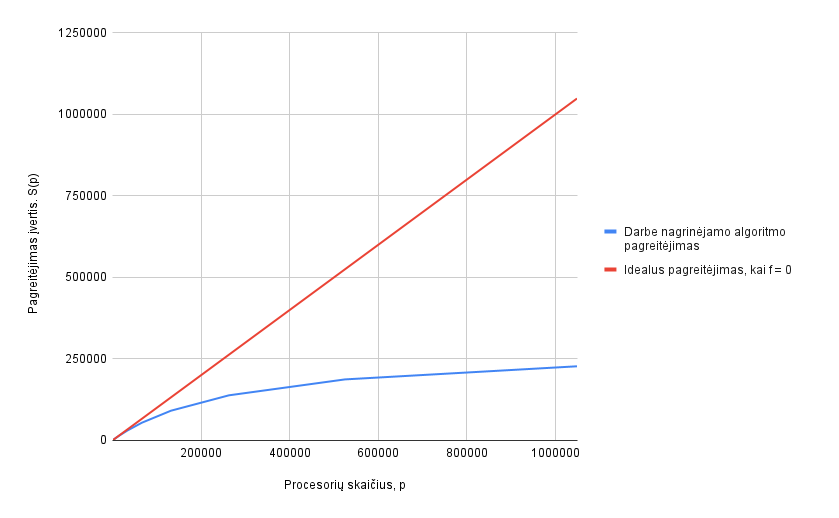
\includegraphics[scale=0.5]{img/max_speedup.png}
    \caption{Maksimalus lygiagretaus algoritmo pagreitėjimo įverčio priklausomybė nuo procesorių skaičiaus}
    \label{img:max_speedup}
\end{figure}

Maksimalaus pagreitėjimo reiškmes naudojant skirtus procesorių kiekius matomos \ref{img:max_speedup} grafike.
Šio darbo ribose algoritmas nebus tiriamas naudojant labai didelį procesorių kiekį, todėl net ir naudojant maksimalų procesorių kiekį (256),
maksimalus pagreitėjimo reikšme bus artima procesorių skaičiui ($S(256) \approx 255.939$), todėl neišlygegretinta algoritmo dalis neribos algoritmo pagreitėjimo.  

Taip pat lygiagretiems algoritmams vertinti naudojama efektyvumo metrika \cite{eager1989speedup}.
Darant prielaidą, kad nuoseklusis algoritmas visada efektyviai išnaudoja jam priskirto procesoriaus resursą, efektyvumo metrika parodo kokia laiko dalį nuoseklusis sprendimas išnaudoja jam priskirtus procesorius.
Efektyvumas, dažniausiai žymimas reide $E$, matematiškai išreiškiamas kaip nuoseklaus algoritmo ir lygiagretaus algoritmo padauginto iš naudotų branduolių skaičiaus vykdymo laiko santykis:

\[ E = \frac{t_s}{t_p * p}\]

Taip pat efektyvumą galime išreikšti per algoritmo pagreitėjimą:

\[ E = \frac{S(p)}{p}\]

Įdealiu atveju, esant maksimaliam algoritmo pagreitėjimui $S(p)=$" algoritmo efektyvumas bus lygus 1. Tai pasiekiama kai visi procesoriai visa laiką yra išnaudojami skaičiavimo užduotims. 


\subsection{Duomenų dalinimas eilutėmis}

Viena iš duomenų paskirstymo lygiagrečiajam algoritmui strategijų yra duomenis paskirstyti eilutėmis (arba stulpeliais).
Norint $N*N$ dydžio matricos duomenis padalint duomenis $p$ procesams, kiekvienam procesui programos vykdymo pradžioje priskiriama po  $(\frac{N-2}{p}+2) * N$ taškų. 
$N-2$ atitinka vidinių matricos stulpelių kiekį, kuris kinta laikui bėgant (2 atitinka išorinius matricos stulpelius turinčius pastovią temperatūrą). 
Ši reikšmė padalinama iš procesų skaičiaus, ir kiekvienas procesui priskiriamos po 2 papildomas eilutes kurios yra naudojamos vidinių reikšmių skaičiavimui (\ref{img:distribution} paveikslėlis).
\begin{figure}[H]
    \centering
    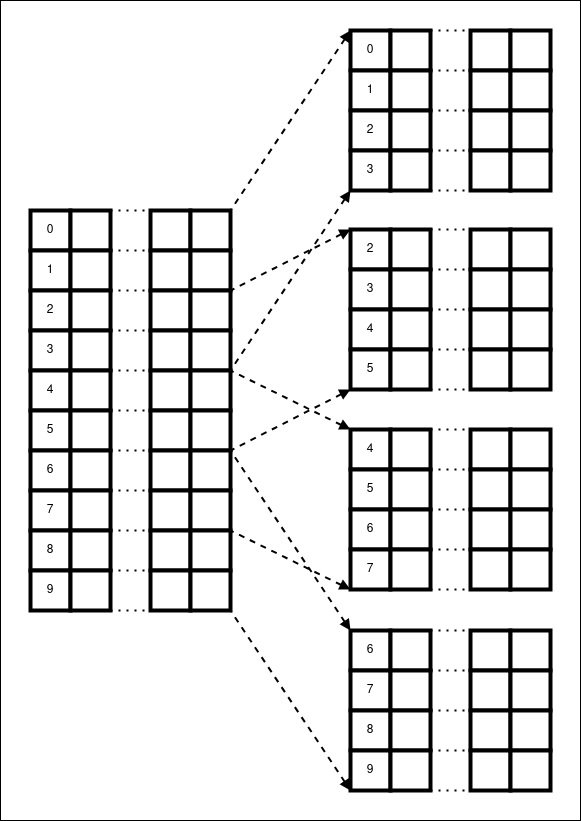
\includegraphics[scale=0.4]{img/distribution.png}
    \caption{Duomenų padalinimas. 10 eilučių padalinamos 4 procesams.}
    \label{img:distribution}
\end{figure}


Naudojant Jakobi iteracinį metodą, kiekvienos iteracijos metu, pirmos ir paskutinės padalintų eilučių reikšmės turi būti sinchronizuojamos tarp gretimas matricos dalis apdorojančių procesų \ref{img:sync}. 
Pirmasis ir paskutinis procesas šonines reikšmės sinchronizuoja tik su vienu iš procesu, nes viena iš jas sudarančių matricos eilučių atitinka pradinės matricos kraštines eilutes, turinčias pastovias reikšmes.

\begin{figure}[H]
    \centering
    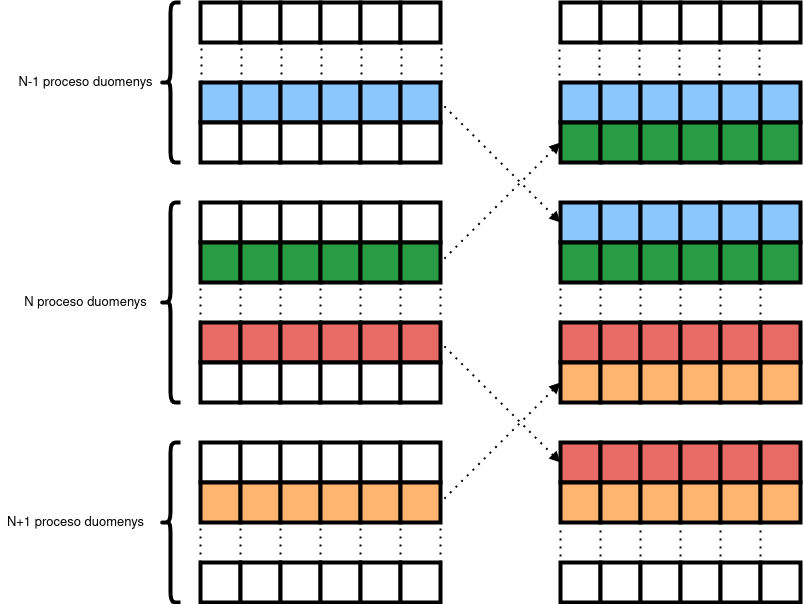
\includegraphics[scale=0.5]{img/sync.png}
    \caption{Duomenų sinchronizacija tarp skirtingų procesų}
    \label{img:sync}
\end{figure}

Norint nustatyti, kada didžiausias temperatūrų iteracijų skirtumas pasiekė norimą reikšmę ir reikia nustoti vykdyti programą, kiekvienoje proceso iteracijos pabaigoje suskaičiuoja didžiausią lokalų temperatūros pokytį ir jį siunčia pagrindiniam procesoriui, 
kuris gavęs visas reikšmes, įvertiną ar bent vienas procesoriaus lokalus skirtumas viršija norima paklaidą, ir nusprendžia ar tęsti iteravimą.
Norint išvengti visuotinio sinchronizavimo tarp visų branduolių ir pagrindinio proceso kiekvienos iteracijos metu, maksimalaus pokyčio reikšmių siuntimas ir palyginimas vykdomas tik kas 1000 iteracijų.

\subsection{Lygiagretaus algoritmo, kai duomenys padalinimo eilutėmis, analyzė}


Lygiagretaus algoritmo veikimo laiko įverčiai, kai matricos kraštinę sudaro 1048 taškų pateikiami \ref{table:parallel1048} lentelėje. 
Prieš testuojant lygiagretųjį algoritmą pakeitus branduolių skaičių, buvo atliekamas testinis paleidimas. 
Testinio paleidimo yra skirtas užtikrinti kad visi užduočiai reikalingi mazgai nebūtų miego būsenoje (ang. Hibernation) ir būtų pasiruošę vykdyti algoritmą.

Kaip matoma \ref{img:parallel_time} grafike, vykdymo laikas atvirkščiai priklauso nuo naudojamų branduolių skaičiaus.

\begin{table}[H]
    \begin{tabular}{|r|r|}
        \hline
        \multicolumn{1}{|l|}{Branduolių skaičius} & \multicolumn{1}{|l|}{Vykdymo laikas (s)} \\ \hline
        2                                         & 1104.232                                 \\ \hline
        4                                         & 571.615                                  \\ \hline
        8                                         & 318.093                                  \\ \hline
        16                                        & 189.300                                  \\ \hline
        32                                        & 106.901                                  \\ \hline
        64                                        & 60.894                                   \\ \hline
        128                                       & 36.370                                   \\ \hline
        256                                       & 21.911                                   \\ \hline
    \end{tabular}
    \caption{Lygiagretaus algoritmo vykdymo laikas, kai matricos kraštinę sudaro 1048 taškų}
    \label{table:parallel1048}
\end{table}

\begin{figure}[H]
    \centering
    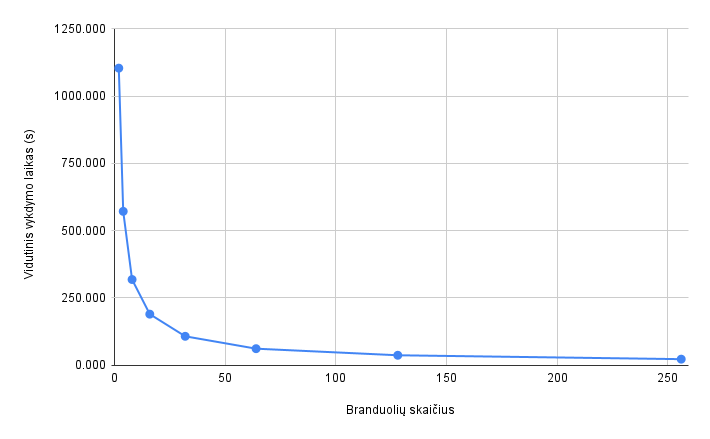
\includegraphics[scale=0.5]{img/parallel_time.png}
    \caption{Lygiagretaus algoritmo vykdymo laiko priklausomybė nuo naudojamų branduolių skaičiaus, kai matricos kraštinę sudaro 1048 taškų}
    \label{img:parallel_time}
\end{figure}


Taip pat lygiagretus algoritmas buvo testuojamas kai matricos kraštinę sudarė 4096 taškai, vykdymo laikas matomas \ref{table:parallel4096} lentelė.
Testuojant naudojant 64 ar mažiau branduolių, programos veikimo laikas viršijo 2 valandas, ir programa buvo sustabdyta. 
Naudojant šią matricos kraštinės reikšmę nuosekliojo algoritmo programa viršydavo sistemos atminties limitą (2GB 1 branduoliui).


\begin{table}[]
    \begin{tabular}{|l|lrrr|}
        \hline
        \multicolumn{1}{|r|}{Branduolių skaičius} & \multicolumn{1}{l|}{Vykdymo laikas (s)} \\ \hline
        \multicolumn{1}{|r|}{128}                 & \multicolumn{1}{r|}{4027.416}           \\ \hline
        \multicolumn{1}{|r|}{256}                 & \multicolumn{1}{r|}{2236.912}           \\ \hline
        
    \end{tabular}
    \caption{Lygiagretaus algoritmo vykdymo laikas, kai matricos kraštinę sudaro 4096 taškai}
    \label{table:parallel4096}
\end{table}



\begin{table}[]
    \begin{tabular}{|r|r|r|r|}
        \hline
        \multicolumn{1}{|l|}{Branduolių skaičius} & \multicolumn{1}{l|}{Vykdymo laikas} & \multicolumn{1}{l|}{Pagreitėjimas, $S(p)$} & \multicolumn{1}{l|}{Efektyvumas, $E(p)=\frac{S(p)}{p}$} \\ \hline
        1                                         & 2155.811                            & 1                                          & 1                                                       \\ \hline
        2                                         & 1104.232                            & 1.952                                      & 0.98                                                    \\ \hline
        4                                         & 571.615                             & 3.771                                      & 0.94                                                    \\ \hline
        8                                         & 318.093                             & 6.777                                      & 0.85                                                    \\ \hline
        16                                        & 189.300                             & 11.388                                     & 0.71                                                    \\ \hline
        32                                        & 106.901                             & 20.166                                     & 0.63                                                    \\ \hline
        64                                        & 60.894                              & 35.402                                     & 0.55                                                    \\ \hline
        128                                       & 36.370                              & 59.275                                     & 0.46                                                    \\ \hline
        256                                       & 21.911                              & 98.390                                     & 0.38                                                    \\ \hline
    \end{tabular}
    \caption{Lygiagretaus algoritmo pagreitėjimas ir efektyvumas. }
    \label{table:speedup}
\end{table}

\begin{figure}[H]
    \centering
    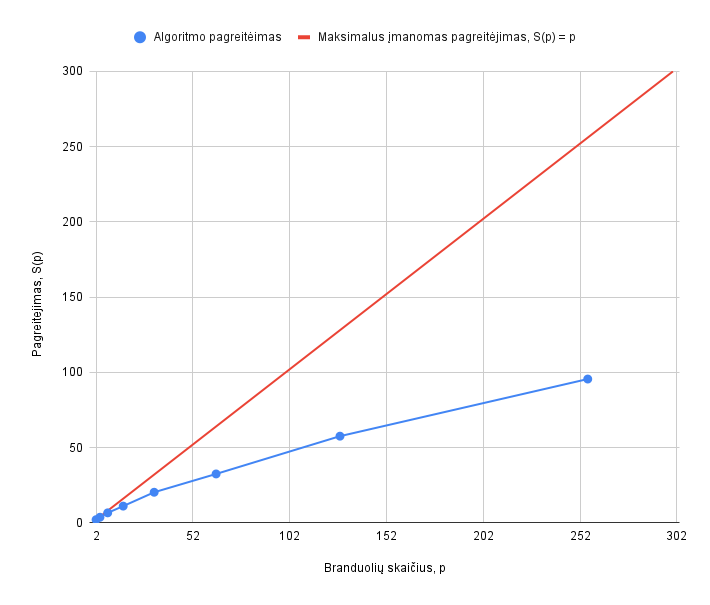
\includegraphics[scale=0.5]{img/parallel_speedup.png}
    \caption{Lygiagretaus algoritmo pagreitėjimo priklausomybė nuo naudojamų branduolių skaičiaus, kai matricos kraštinę sudaro 1048 taškų}
    \label{img:parallel_speedup}
\end{figure}


\ref{img:parallel_speedup} grafike matomas lygiagretaus algoritmo logaritminis pagreitėjimas, tačiau Amdahl'o dėsnio \cite{amdahl1967validity} apibrėžiamas maksimalus pagreitėjimas nėra pasiekiamas - naudojant tokį branduolių kiekį pagreitėjimas turėtų būti artimas idealiam pagreitėjimui  $S_{max}(p)=p$.
Tai galimai nutinka dėl to, kad Amdahl'o dėsnis neatsižvelgia į komunikacijos tarp skirtingų procesorių kaštus.
Tikslų programos skaičiavimų ir komunikacijos santykį įvertinti yra sunku, nes komunikacijos laikas gali skirtis laikas priklausomai ar komunikuojantys procesai naudoja to pačio ar skirtingų centrinių procesorių branduolius, 
ir ar centriniai procesoriai yra toje pačioje ar skirtinguose motininėse plokštelėse. 
Tas iš dalies matoma \ref{table:speedup} lentelėje, kad algoritmo efektyvumas naudojant 2 ir 4 branduolius yra artimas 1, o naudojant daugiau branduolių lygiagretaus sprendimo efektyvumas mažėja.
Tai galima sieti su tuo kad testavimui naudoto paskirstytų skaičiavimų tinklo mazguose naudojami procesoriai, turinys 6 branduolius, todėl naudojant 2 ir 4 branduolius didelė tikimybė, kad bus naudojamas 1 fizinis procesorius, taip išvengiant didelių komunikacijos kaštai tarp atskirų procesų.
Taip pat, \ref{table:speedup} lentelėje matomas algoritmo efektyvumo mažėjimas didinant branduolių skaičių, iš to galime daryti prielaidą, kad pradinius duomenis skaidant į vis mažesnes dalis, vis didesnę algoritmo vykdymo laiką užima komunikacija tarp skirtingus duomenis apdorojančių procesų.
Nors testuojant su vis didesnių branduolių skaičiumi algoritmo efektyvumas mažėja, lygiagretaus algoritmo pagreitėjimo metrika didinant naudojamų branduolių nenustoja didėti, iš to galima daryti prielaidą šių testų metu nebuvo rastas branduolių skaičius, kurį naudojant komunikacijos kaštai nusvertų gautą algoritmo pagreitėjimą, kai užduotis yra padalinama į mažesnes dalis. 

% Medžiagos darbo tema dėstymo skyriuose pateikiamos nagrinėjamos temos detalės: pradinė me-
% džiaga, jos analizės ir apdorojimo metodai, sprendimų įgyvendinimas, gautų rezultatų apibendrinimas.
% Šios dalies turinys labai priklauso nuo darbo temos. Kursiniame darbe analizuojama dalykinė sritis, jo
% rezultate formuluojamas bakalauro darbe sprendžiamas uždavinys. Referatas neatitinka kursiniams
% darbams keliamų reikalavimų. Dėstymo skyriai gali turėti poskyrius ir smulkesnes sudėtines dalis, kaip
% punktus ir papunkčius

% Medžiaga turi būti dėstoma aiškiai, pateikiant argumentus. Tekste dėstomas
% trečiuoju asmeniu, t.y. rašoma ne „aš manau“, bet „autorius mano“, „autoriaus
% nuomone“. Reikėtų vengti informacijos nesuteikiančių frazių, pvz., „...kaip jau
% buvo minėta...“, „...kaip visiems žinoma...“ ir pan., vengti grožinės
% literatūros ar publicistinio stiliaus, gausių metaforų ar panašių meninės
% išraiškos priemonių.

\section{Lygiagretusis algoritmas, naudojantis grafinius procesorius}


Lygiagrečiam algoritmui sukurti naudojančiam grafinius procesorius buvo naudota C++ kalbos CUDA biblioteka \cite{yang2008parallel}. 
Algoritmo pradžioje alokuojama atmintis trims N*N dydžio masyvams, kur N yra matricos kraštinės ilgis. 
Dviejuose masyvuose, kaip nuosekliąjį algoritmą įgyvendinančiojoje programoje, saugoma dabartinė matricos būsena ir pildomos naujomis reikšmėmis iteracijos metu, o trečiasis yra skirtas saugoti temperatūrų skirtumui tarp iteracijų ir yra naudojamas galutinės pakaidos skaičiavimui.
Programos vykdymo pradžioje, kaip ir nuosekliajame algortime, pirmasis masyvas užpildomas pradine matricos būsena.
Kadangi naudojamas grafinis procesorius, kuris yra skirtas operuoji savo atmintyje esančia infromacija, visų tris masyvams reikia išskirti atminties vieta GPU atmintyje ir ten nukopijuoti duomenis iš bendrosios paskirties atminties.

Kaip ir nusekliajame algoritme tada pradedamas iteracinis procesas, kai kiekvienos iteracijos metu, kiekvienam vidiniam matricos taškui yra priskiriama reikšmė, lygi jį supančių 4 taškų vidurkiui, o kraštinės matricos reikšmės nekinta.
Taip pat iteracijos metu į atskirą matricą fiksuojamas maksimalus temperatūros pasikeitimas, skirtas nustatyti ar temperatūros pasiskirstymas pasiekė galutinė savo būseną.
Kas 1000 iteracijų šios matricos reikšmės yra nukopijuojamos iš grafinės prokštės atminties į bendrąją atmintį, taip gražinant jos reikšmes į pagrindinį procesą. 
Tada pagrindinis procesas, naudodamas centrinio procesoriaus resursus, randa didžiausia matricos reikšmė ir ji yra palyginama su konfiguracijos faile nustatyta paklaidos reikšme.
Jei temperatūros pasikeitimas yra mažesnis už numatytąją paklaida, laikome kad matrica pasiekė savo galutinį temperatūrų pasiskirstymą, ir temperatūros matricos reikšmės yra nukopijuojamos iš grafinės prokštės atminties į bendrąją atmintį. 

Prieš paleidžiant kodą, konfiguraciame faile nurodomas duomenų pasiskirstymas.
CUDA programoms duomenų paskirtymui naudojami du parametrai blokų kiekis ir gijas per bloką.
Kiekvieno bloko duomenys yra apdorojimi vieno iš GPU srautinių apdorojimo proceriaus (ang. streaming multiprocessor - SM).  
Kadangi kiekvienos iteracijos metu aprodojami turi būti visi duomenys, bendras gijų kiekis turi atitikti matricos taškų kiekį: 

\[ Bloku\_skaicius \times giju\_skaicius\_per\_bloka = N \times N  ,\]

kur $N$ yra matricos dimensija.


\begin{table}[]
    \begin{tabular}{|r|r|r|r|}
        \hline
        \multicolumn{1}{|l|}{Gijų skaičius per bloką} & \multicolumn{1}{l|}{Blokų skaičius} & \multicolumn{1}{l|}{Vykdymo laikas, s} & \multicolumn{1}{l|}{Pagreitėjimas, kartais} \\ \hline
        1                                             & 1048576                             & 237.355                                & 9.1                                         \\ \hline
        2                                             & 524288                              & 118.921                                & 18.1                                        \\ \hline
        4                                             & 262144                              & 59.709                                 & 36.1                                        \\ \hline
        8                                             & 131072                              & 29.8363                                & 72.3                                        \\ \hline
        16                                            & 65536                               & 15.492                                 & 139.2                                       \\ \hline
        32                                            & 32768                               & 8.325                                  & 259.0                                       \\ \hline
        64                                            & 16384                               & 6.05                                   & 356.3                                       \\ \hline
        128                                           & 8192                                & 6.026                                  & 357.8                                       \\ \hline
        256                                           & 4096                                & 6.03                                   & 357.5                                       \\ \hline
        512                                           & 2048                                & 5.984                                  & 360.3                                       \\ \hline
        1024                                          & 1024                                & 6.097                                  & 353.6                                       \\ \hline
    \end{tabular}
    \caption{Lygiagretaus algoritmo naudojančio GPU vykdymo laikas naudojant skirtingus blokų ir gijų per bloką parametrus, kai matricos kraštinę sudaro 1048 taškų}
    \label{table:gpu_threads}
\end{table}


\begin{figure}[H]
    \centering
    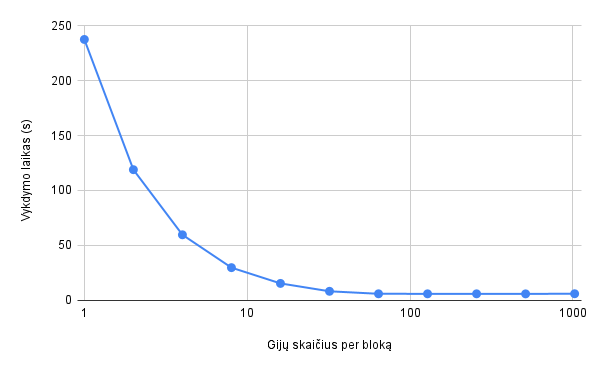
\includegraphics[scale=0.7]{img/gpu_threads.png}
    \caption{Lygiagretaus algoritmo naudojančio GPU vykdymo Lygiagretaus algoritmo naudojančio GPU vykdymo laiko priklausomybė nuo gijų per bloką skaičiaus}
    \label{img:gpu_threads}
\end{figure}


Priešingai nei testuojant lygiagretųjį algorimtą naudojantį centrinius procesorius, naudojamų gijų skaičius nebuvo ribojamas - buvo naudoja visi grafinio procesoriaus pajėgumai.
Šilumos uždavinio lygiagretinimo rezultatai naudojant grafinį procesorių su skirtingas blokų ir gijų per bloką parametrus, o matricos kraštinė yra lygi 1024 taškams, yra pateikiami \ref{table:gpu_threads} lentelėje. 
Matoma, kad naudojant GPU pasiektas pagreitėjimas iki 360 kartų lyginant su nuosekliuoju CPU naudojančiu algoritmų.

Kaip matoma \ref{img:gpu_threads} grafike, lygiagretusis algoritmas veikia daug lečiau jei yra naudojami mažiau nei 32 gijos per bloką. 
Tai galima sieti su tuo kad CUDA architektūroje kiekvienas procesorius vykdo vieną komandą 32 gijoms iš karto, todėl naudojant mažiau nei 32 gijas nėra pilnai išnaudojamos procesoriaus galimybes.
Naudojant daugiau gijų nėra pasiekiamas geresnis rezultatas, nes šio uždavinio GPU implementacijos skaičiavimuose yra naudojama tik bendra atmintis, todėl nėra išnaudojamas blokuose esanti greitesnė dedikuota atmintis. 
Naudoti daugiau nei 1024 gijas per bloką neleidžia CUDA architetūra.


\begin{table}[]
    \begin{tabular}{|r|r|r|r|}
        \hline
        \multicolumn{1}{|l|}{Matricos kraštinės ilgis} & \multicolumn{1}{l|}{Vykdymo laikas, s} & \multicolumn{1}{l|}{Iteracijų skaičius} & \multicolumn{1}{l|}{10000 iteracijų vykdymo laikas} \\ \hline
        128                                            & 0.063                                  & 17000                                   & 0.037                                               \\ \hline
        256                                            & 0.175                                  & 49000                                   & 0.035                                               \\ \hline
        512                                            & 0.783                                  & 122000                                  & 0.064                                               \\ \hline
        1024                                           & 5.643                                  & 156000                                  & 0.361                                               \\ \hline
        2048                                           & 21.463                                 & 155000                                  & 1.384                                               \\ \hline
        4196                                           & 94.393                                 & 168000                                  & 5.618                                               \\ \hline
        8392                                           & 463.99                                 & 210000                                  & 22.094                                              \\ \hline
    \end{tabular}
    \caption{Lygiagretaus algoritmo naudojančio GPU vykdymo laikas naudojant 512 gijas per bloką}
    \label{table:gpu_dim}
\end{table}

Taip pat grafinių procesorių greitaveika buvo tiriama naudojant skirtingus matricų kraštinių reikšmes.
Kaip matoma \ref{table:gpu_dim} lentelėje, naudojant mažas matricų kraštinių ilgio reikšmes (iki 512), 10000 iteracijų vykdymo greitis nekinta, tačiau toliau didinant matricos kraštinių reikšmės 10000 iteracijų vykdymo laikas didėja logoritmiškai, kaip ir nuosekliajame algortime.
Iš to galima daryti išvadą, kad GPU skaičiavimuose naudojant mažą duomenų kiekį, didelę programos vykdymo laiko dalį užima GPU branduolių ir duomenų kopijavimo inicijavimas. 

Šiame darbe implementuotą grafinius procesorius naudojantį algoritmą galime palyginti su kitame šilumos laidumo lygties sprendimą nagrinėjančiu darbe \cite{belhaous2021comparative} aprašytu algoritmu. 
Kitame darbe \cite{belhaous2021comparative} algoritmas buvo testuojamas naudojant $5120 \times 5120$ ir $20000 \times 20000$ dydžio matricas, tačiau programa buvo vykdoma tik ribota iteracijų skaičių - 5000 ir algoritmo vykdymas užtruko atitinkamai 8.85 ir  141.11 sekundžių.
Testuojant šio darbo rašymo metu implementuotą algoritmą su tokias pačiais parametrais, algoritmo vykdymo laikas užtruko atitinkamai 4.142 ir 62.31 sekundes.
Pagal lyginamajame darbe \cite{belhaous2021comparative} aprašytą grafinę plokštę ir naudojamų CUDA branduolių skaičių galime, nustatyti kad jame buvo naudojami viengubo tikslumo slankaus kablelio - 32 bitų  skaičiai.
Šiame darbe atliktuose testuose yra naudojami dvigubo tikslumo slankaus kablelio - 64 bitų skaičiai.
Perrašius šio darbo algoritmą, kad jis naudotų viengubo tikslumo slankaus kablelio skaičius, programos vykdymo laikai atinkamai sutrumpėjo iki 2.152 ir 32.871 sekundžių, ką galime sieti su tuo kad V100 vaizdo plokštė turi dvigubai daugiau 32 bitu slankaus kablelio skaičius procesorių.    
Matoma kad šio darbe atliktų testų metu grafines plokštes naudojantis algoritmas veikia daugiau nei 4 kartus greičiau.
Ši laiko skirtumą galima sieti kad šio darbo metu buvo naudotas naujesnis ir galingesnis grafinis procesorius turintis 4 kartus daugiau CUDA branduolių, taip pat skirtumą galėjo paveikti ir algoritmų implementacijų skirtumai.
Atsižvelgdami į tai, galime tvirtinti kad darbe nagrinėjamas grafinius procesorius naudojantis algoritmas veikia korektiškai.


\section{Grafinius ir centrinius procesorius naudojančių algortimų palyginimas}

Norint palyginti GPU ir CPU reikia įsivesti vertinimo kriterijus.

Vienas vertinimo kriterijus yra vykdymo laikas.
Jis yra svarbus kai vykdoma užduoties sprendimas yra jautrus laikui \cite{yang2019re}. 
Vienas tokio vertinimo minusų yra neatsižvelgimas į skaičiavimo kaštus - naudojant didesnį skaičiavimo resursų kiekį dažniausiai bus pasiekiamas greitesnis rezultatas.

Dažnai GPU ir CPU algoritmo palyginuose vykdymo laiko metrija yra CPU ir GPU branduolių skaičiumi \cite{garland2008parallel, belhaous2021comparative}.
Toks palyginimas nėra visiškai korektiškas nes CPU ir GPU branduoliai skiriasi savo architektūra, veikimo greičiu ir paskirtimi, o ir skirtingų kartų įrenginiai skiriasi skaičiavimo galimybėmis (ang. compute capability) ir veikimo greičiu.

Dar vienas būdas lyginti centrinių ir grafinių procesorių veikimo efektyvumą yra matuoti algortimo veikimo metu naudojama energiją.
Tai leistų praktiškai įvertini sunaudotos elektros energijos kaštus duomenų centrui. 
Šiame darbe atliktų eksperimentų metu naudotos elektros energijos kaštų informacija nėra prieinama, todėl kaštai bus vertinami teoriškai.

Ekperimentų metu naudojamas V100 grafinis procesorius esant pilnai apkrovai gali naudoti 300W energijos.
Centrinių procesorių naudojamos energijos kiekis priklauso atliekamos užduoties \cite{von2016variations}, todėl vertinimui naudosime gamintojo pateikiama TDP vertę, kuri Xeon X5650 atveju yra 95W.
Skaičiamu metu laikysime kad likusieji mazgų komponentai skaičiavimų metu naudoja 100W energijos, o rezultatą norime gauti maksimaliai greitai.

Lygiagrečiajam algoritmui, naudojančiam grafinius procesorius, vykdyti bus reikalingas vienas mazgas su dviems centriniais procesoriams ir vienu grafiniu procesoriumi.
Darydami prielaidą kad sistema ekperimento metu bus pilnai apkrauta, galime apytiksliai numatyti ši sistema per vieną skaičiavimų sekundę sunaudotos $100+300+95\times2 = 590$ Vatų energijos.
Kadangi geriausiais algoritmas buvo vykdomas 6s sekundes, tai sistema su GPU skaičiavimu metu sunaudos $590\times6 = 3540$ Džaulius energijos.

Lygiagrečiajam algoritmui, naudojančiam centrinius procesorius, vykdyti bus reikalingas 22 mazgai su dviems centriniais procesoriams.
Ši sistema apytiksliai per vieną skaičiavimų sekundę sunaudotos $(100+95\times2)\times22 = 6160$ Vatų energijos.
Kadangi geriausiais algoritmas buvo vykdomas 21s sekundes, tai sistema naudodama tik centrinius procesorius skaičiavimu metu sunaudos $6160\times21 = 129360$ Džaulius energijos.

Pagal šiuos skaičiavimus galima matyti kad grafiniai procesoriai šilumos pasiskirtymo uždavinio sprendimui sunaudos mažesnį energijos kiekį.

\sectionnonum{Rezultatai}

\begin{itemize}
    \item Implementuoti nuoseklusis ir lygiagretusis centrinius procesorius naudojantys algoritmai  spendžiantys šilumos pasiskirstymo užduotį Jacobi iteraciniu metodu naudojant baigtinių skirtumų schemą.
    \item Atliktas lygiagretaus algoritmo, naudojančio centrinius procesorius, efektyvumo ir teorinio ir praktinio pagreitėjimo analyzė.
    \item Implementuotas lygiagretusis šilumos pasiskirstymo uždavinį sprendžiantis algortimas naudojantis grafinius procesorius.
    \item Algoritmai buvo ištestuoti naudojant Vilniaus Universiteto Matematikos ir Informatikos fakulteto Skaitmeninių tyrimų ir skaičiavimų centro paskirstytų skaičiavimų tinklo resursus.
          Naudojant 256 centrinius procesorius buvo pasiektas 98 kartų pagreitėjimas, o naudojant 1 Nvidia Tesla V100-SXM2 32GB grafinį procesorių buvo pasiektas 360 kartų pagreitėjimas.
    \item Atliktas algoritmo, naudojančio grafinius procesorius, vykdymo laiko palyginimas su tokį pati uždavinį sprendžiančiu darbu \cite{belhaous2021comparative} ir gautas ekvivalentus rezultatas.
\end{itemize}

\sectionnonum{Išvados}
\begin{itemize}
    \item Sprendžiant šilumos pasiskirstymo uždavinį pasiskirtytų skaičiavimo tinkle naudojant centrinius procesorius komunikacija tarp skirtingu tinklo mazgų lėtiną algoritmo veikimą.
    \item Norint gauti geresnius centrinius procesorius naudojančio lygiagretaus algoritmo pagreitėjimo ir efektyvumo rezultatus, būtų verta pabandyti kitokius duomenų dalinimo būdus (pvz. kvadratais), didinti procesorių skaičių mazguose.
    \item Grafiniai procesoriai leidžia greičiau ir naudojant mažiau energijos resursų išspresti šilumos pasiskirstymo uždavinį nei to šio uždavinio sprendimas naudojant centrinius procesorius.
    \item Norint padidinti grafinius procesoriaus naudojančio algoritmo veikimo greitį, būtų verta pabandyti naudoti grafinių plokščių blokuose esančią dedikuotą atmintį, naudoti daugiau nei vieną vaizdo plokštę.
\end{itemize}
% Darbo uždaviniai:
% \begin{itemize}
%     \item implementuoti nuoseklųjį algoritmą, sprendžianti šilumos pasiskirstymo uždavinį
%     \item implementuoti nuseklu ir įvertinti šilumos laidumo uždavinio algoritmo pagreitėjimą naudojant centrinius procesorius
%     \item suprojektuoti ir implementuoti šilumos laidumo uždavinio sprendimo algorimtą, naudojantį grafinių procesorių resursus
%     \item įvertinti grafinius procesorius naudojančio algoritmo našumą ir praktiškumą lyginant su centrinius procesorius naudojančiu algoritmu
%     \item palyginti gautus rezultatus rezultatus su kitais panašiais problemas nagrinėjančių mokslinių darbų rezultatais
% \end{itemize}

% Darbo rezultatai:
% \begin{itemize}
%     \item Nuoskelioji šilumos laidumo uždavinio sprendimo implementacija
%     \item Lygiagrečioji šilumos laidumo uždavinio algoritmo sprendimo naudojanti centrinius procesorius
%     \item Lygiagrečioji laidumo uždavinio sprendimo implementacija naudojanti grafinius procesorius
%     \item Algoritmų teorinių ir praktinių pagreitėjimų analyzė
%     \item Grafinius ir centrinius procesorius naudojančių algoritmų pagreitėjimų palyginimas
% \end{itemize}


% kuriame pateikiami tyrimo objektas ir aktualumas, darbo tikslas, keliami už-
% daviniai ir laukiami rezultatai, tyrimo metodai, numatomas darbo atlikimo procesas, apibūdi-
% nami darbui aktualūs literatūros šaltiniai.
% Pastaba. Darbo uždavinyje apibrėžiamas siekiamas rezultatas, kad būtų galimybė išmatuoti,
% ar tikslai ir uždaviniai yra išspręsti, bei kokiu lygiu (vertinant kiekybę bei kokybę). Pavyz-
% džiui, „Atlikti literatūros .... analizę“ nėra tinkamas uždavinys, nes nusako procesą, tačiau
% neapibrėžia jo rezultato. Tinkamos uždavinio formuluotės šablonai: „Išanalizuoti literatūrą
% ... siekiant apžvelgti ir įvertinti /... metodų tinkamumą sprendžiamam uždaviniui/privalu-
% mus ir trūkumus sprendžiant ... uždavinį/rekomenduojamas ... projektavimo gaires, šablonus
% ir pan.

% \sectionnonum{Įvadas}
% Įvade nurodomas darbo tikslas ir uždaviniai, kuriais bus įgyvendinamas tikslas,
% aprašomas temos aktualumas, apibrėžiamas tiriamasis objektas akcentuojant
% neapibrėžtumą, kuris bus išspręstas darbe, aptariamos teorinės darbo prielaidos
% bei metodika, apibūdinami su tema susiję literatūros ar kitokie šaltiniai,
% temos analizės tvarka, darbo atlikimo aplinkybės, pateikiama žinių apie
% naudojamus instrumentus (programas ir kt., jei darbe yra eksperimentinė dalis).
% Darbo įvadas neturi būti dėstymo santrauka. Įvado apimtis 2 -- 4 puslapiai.

% \section{Medžiagos darbo tema dėstymo skyriai}
% Medžiagos darbo tema dėstymo skyriuose išsamiai pateikiamos nagrinėjamos temos
% detalės: pradiniai duomenys, jų analizės ir apdorojimo metodai, sprendimų
% įgyvendinimas, gautų rezultatų apibendrinimas.


% Skyriai gali turėti poskyrius ir smulkesnes sudėtines dalis, kaip punktus ir
% papunkčius.




% \sectionnonum{Rezultatai ir išvados}
% Rezultatų ir išvadų dalyje turi būti aiškiai išdėstomi pagrindiniai darbo rezultatai (kažkas išana-
% lizuota, kažkas sukurta, kažkas įdiegta) ir pateikiamos išvados (daromi nagrinėtų problemų sprendimo
% metodų palyginimai, teikiamos rekomendacijos, akcentuojamos naujovės).

\printbibliography[heading=bibintoc]  % Šaltinių sąraše nurodoma panaudota
% literatūra, kitokie šaltiniai. Abėcėlės tvarka išdėstomi darbe panaudotų
% (cituotų, perfrazuotų ar bent paminėtų) mokslo leidinių, kitokių publikacijų
% bibliografiniai aprašai. Šaltinių sąrašas spausdinamas iš naujo puslapio.
% Aprašai pateikiami netransliteruoti. Šaltinių sąraše negali būti tokių
% šaltinių, kurie nebuvo paminėti tekste. Šaltinių sąraše rekomenduojame
% necituoti savo kursinio darbo, nes tai nėra oficialus literatūros šaltinis.
% Jei tokių nuorodų reikia, pateikti jas tekste.

% \sectionnonum{Sąvokų apibrėžimai}
% \sectionnonum{Santrumpos}
% Sąvokų apibrėžimai ir santrumpų sąrašas sudaromas tada, kai darbo tekste
% vartojami specialūs paaiškinimo reikalaujantys terminai ir rečiau sutinkamos
% santrumpos.

\end{document}
